% Bản dịch tiếng Việt để rà soát nội dung — compile bằng XeLaTeX.
\documentclass[conference]{IEEEtran}
\IEEEoverridecommandlockouts
\usepackage{fontspec}
\setmainfont{Times New Roman}
\usepackage{cite}
\usepackage{amsmath,amssymb,amsfonts}
\usepackage{graphicx}
\usepackage{xcolor}
\usepackage{booktabs}
\usepackage{multirow}
\usepackage{placeins}
\usepackage{enumitem}
\usepackage{hyperref}
\hypersetup{hidelinks}
\usepackage{tikz}
\usetikzlibrary{arrows.meta,positioning,calc}

\renewcommand{\figurename}{Hình}
\renewcommand{\tablename}{Bảng}
\renewcommand{\refname}{Tài liệu tham khảo}

\newcommand{\wasm}{\textnormal{\textsc{wasm}}}
\newcommand{\ms}{\,ms}

\definecolor{hwblue}{RGB}{180,205,240}
\definecolor{osbrown}{RGB}{255,200,100}
\definecolor{wgreen}{RGB}{144,220,144}
\definecolor{cpurple}{RGB}{210,185,235}
\definecolor{cblue}{RGB}{150,195,235}
\definecolor{yorange}{RGB}{220,155,130}
\definecolor{gpink}{RGB}{255,200,200}

\begin{document}

\title{Điện toán biên trên nền Web cho Nhận dạng Dấu Quang học:\protect\\
Một đánh giá hiệu năng đa nền tảng}

\author{%
\IEEEauthorblockA{%
Khoa Hệ thống Thông tin\\
Trường Đại học Công nghệ Thông tin, ĐHQG-HCM\\
Thành phố Hồ Chí Minh, Việt Nam}
\vspace{0.35em}
\IEEEauthorblockN{%
\begin{tabular}{@{}c@{\hspace{2.6em}}c@{\hspace{2.6em}}c@{}}
Phan Huy Kiên & Trương Minh Châu & Nguyễn Thanh Bình
\end{tabular}}
\IEEEauthorblockA{%
\begin{tabular}{@{}c@{\hspace{2.6em}}c@{\hspace{2.6em}}c@{}}
\texttt{huykien283@gmail.com} & \texttt{chautm@uit.edu.vn} & \texttt{binhnt@uit.edu.vn}
\end{tabular}}
}

\maketitle

\begin{abstract}
Nhận dạng Dấu Quang học (Optical Mark Recognition, OMR) chạy trên trình
duyệt có thể giữ phiếu trả lời của học sinh ngay trên thiết bị và không
cần cài đặt ứng dụng, nhưng chi phí của nó phân bố ra sao theo từng giai
đoạn xử lý và theo từng nền tảng thì chưa được đo đạc. Bài báo này đóng
góp một benchmark đa nền tảng cho một pipeline OMR Web Edge hoàn chỉnh,
ghép thị giác máy tính bằng WebAssembly (\wasm{}) với suy luận YOLO trên
WebGPU, đo so với một mốc Native Android trên bộ ngữ liệu 179 phiếu đã
được con người rà soát và bảy nền tảng Web. Chúng tôi báo cáo độ chính
xác nhận dạng, độ trễ theo từng giai đoạn, và mức dùng tài nguyên cho hai
cấu hình có thể hoán đổi: một pipeline chỉ-CV đạt độ chính xác câu hỏi
99,00\%, và một bộ phát hiện YOLO theo điểm-góc (corner keypoint) đưa bốn
điểm mốc dự đoán vào phép biến đổi homography và đạt 99,43\% trên bốn
thiết bị; để đối chiếu, dùng chính bộ phát hiện đó dưới dạng cắt theo hộp
bao (bounding-box) đo được 63,70--74,40\%. Dữ liệu độ trễ định vị rõ chi
phí: trên cùng thiết bị Redmi, lõi CV trên \wasm{} chậm hơn Native
$6,1\times$ ($466$ so với $77$\,ms), so với chỉ $3,6\times$ giữa suy luận
WebGPU và NNAPI. Các phép đo này cho thấy WebGPU đã hạ suy luận YOLO xuống
chi phí thứ yếu, trong khi giai đoạn CV tất định chạy qua \wasm{} mới chi
phối độ trễ đầu-cuối, nên một hệ OMR Web Edge có tính cạnh tranh phụ thuộc
vào việc giảm chi phí CV trên \wasm{} chứ không phải vào việc tăng tốc bộ
phát hiện.
\end{abstract}

\begin{IEEEkeywords}
Nhận dạng dấu quang học, điện toán biên, trình duyệt web, YOLO,
WebAssembly, WebGPU, đánh giá hiệu năng đa nền tảng
\end{IEEEkeywords}

\section{Giới thiệu}

Việc chấm tự động các phiếu trắc nghiệm được sử dụng rộng rãi trong các
cơ sở giáo dục, nơi khối lượng lớn phiếu phải được xử lý chính xác trong
thời gian ngắn. Các triển khai hiện có theo hai khuôn mẫu đã được khẳng
định. Các dịch vụ dựa trên máy chủ truyền ảnh quét hoặc chụp lên hạ tầng
từ xa, kéo theo sự phụ thuộc vào mạng và làm lộ dữ liệu học sinh ra các hệ
thống bên ngoài~\cite{patel2015,okorie2022}. Các ứng dụng di động bản địa
tránh được việc truyền dữ liệu nhưng đòi hỏi đóng gói riêng theo nền tảng,
phân phối qua kho ứng dụng, và chi phí bảo trì cho từng nền tảng.

Sự trưởng thành gần đây của \wasm{} và WebGPU nay cho phép các tác vụ thị
giác máy tính và học sâu thực thi trực tiếp bên trong các trình duyệt
hiện đại mà không cần plugin hay cài đặt, qua đó mở ra một mô hình triển
khai thứ ba: một pipeline hoàn toàn phía máy khách, trong đó ảnh phiếu trả
lời được xử lý ngay trong trình duyệt và không bao giờ rời khỏi thiết bị.
Vì một gói mã duy nhất triển khai qua URL phục vụ được cả trình duyệt
desktop lẫn di động, mô hình này tránh được rủi ro lộ dữ liệu vốn có của
việc chấm phía máy chủ, đồng thời loại bỏ trở ngại cài đặt của một ứng
dụng bản địa.

Trong trình duyệt, các tải công việc này ánh xạ lên hai nền tảng thực thi
khác nhau. Các giai đoạn xử lý ảnh cổ điển — cụ thể là nắn chỉnh phối
cảnh, ngưỡng hóa thích nghi, và đọc ô tròn theo lưới cố định — được biên
dịch từ C\texttt{++}/OpenCV sang \wasm{} và chạy trên CPU, trong khi việc
định vị vùng phiếu có thể tùy chọn được giao cho suy luận nơ-ron qua ONNX
Runtime Web trên một backend WebGPU. Như vậy, một bản triển khai có thể
chạy pipeline chỉ-CV hoặc bổ sung một bộ phát hiện YOLO cho bước định vị;
vì hai nền tảng này dùng các API trình duyệt và phần cứng khác nhau, chính
chi phí tương đối của chúng — chứ không phải riêng một thành phần nào — mới
quyết định liệu một cấu hình cho trước có thể sánh được với thực thi bản
địa hay không. Benchmark này đo cả hai.

Theo đó, bài báo này đặt câu hỏi liệu suy luận WebGPU, tự thân nó, có đủ
để làm cho một pipeline OMR Web Edge cạnh tranh được với Native Android
hay không. Dưới khối lượng công việc đo được, câu trả lời là không: WebGPU
có làm giảm độ trễ YOLO, nhưng giai đoạn CV/\wasm{} tất định sau đó lại
chi phối hành vi đầu-cuối. Điều này khiến Native Android vẫn là phương án
triển khai có độ trễ thấp hơn, trong khi Web Edge là lựa chọn bảo toàn
quyền riêng tư và triển khai qua URL, mà tính cạnh tranh phụ thuộc vào
việc kìm giữ giai đoạn CV trên \wasm{}.

Bài báo có ba đóng góp:
\begin{enumerate}[leftmargin=*, itemsep=1pt, topsep=2pt]
  \item Một đánh giá OMR đa nền tảng đã rà soát trên bộ 179 phiếu, với các
  phép đo độ chính xác có giám sát, độ trễ và tài nguyên trên bảy nền tảng
  Web Edge và một mốc Native Android.
  \item Một kết quả quy gán theo giai đoạn cho thấy OMR trên \wasm{}, chứ
  không phải suy luận YOLO, mới là nút thắt cổ chai chủ đạo: trên cùng
  thiết bị Redmi, khoảng cách \texttt{cpp\_ms} của CV giữa Mobile Web và
  Native là $6,1\times$ ($466$ so với $77$\,ms), trong khi khoảng cách suy
  luận giữa WebGPU và NNAPI chỉ là $3,6\times$ ($541$ so với $150$\,ms).
  \item Một công thức theo điểm-góc biến YOLO thành bộ phát hiện chính đã
  kiểm chứng: đưa thẳng bốn điểm mốc góc dự đoán vào homography đạt
  99,43\% trên bốn thiết bị, vượt mốc CV 99,00\%, trong khi cách cắt theo
  hộp bao ngây thơ của cùng bộ phát hiện lại sụp còn 63,70--74,40\%.
\end{enumerate}

\section{Các công trình liên quan}

\paragraph{OMR cổ điển}
Các pipeline OMR truyền thống dựa vào các kỹ thuật xử lý ảnh thủ công như
ngưỡng hóa, dò biên, và các phép toán hình thái để định vị và nhận dạng ô
tròn~\cite{patel2015,okorie2022}. Tuy hiệu quả về mặt tính toán, các
phương pháp này vẫn nhạy cảm với biến thiên ánh sáng và méo hình học trong
các tình huống chụp bằng thiết bị di động~\cite{afifi2019}.

\paragraph{Học sâu cho OMR}
Các nghiên cứu gần đây áp dụng các bộ phát hiện dựa trên
YOLO~\cite{redmon2016} để tăng độ bền vững trong điều kiện chụp khó khăn.
Ali và cộng sự~\cite{ali2025} cho thấy YOLO đạt độ chính xác phát hiện cao
hơn và tổng quát hóa tốt hơn so với các phương pháp dựa trên ngưỡng, trong
khi YOLOv8n~\cite{jocher2023} cung cấp một kiến trúc nhẹ phù hợp cho triển
khai biên. Tabassum và Rahman~\cite{tabassum2024} triển khai YOLOv8 cho
OMR di động nhưng không báo cáo phân rã độ trễ theo giai đoạn lẫn so sánh
đa nền tảng có kiểm soát, để ngỏ việc chi phí suy luận liên hệ thế nào với
pipeline CV xung quanh trên các thiết bị hạn chế.

\paragraph{Điện toán biên trên nền trình duyệt}
\wasm{} và WebGPU cùng nhau cho phép thực thi phía máy khách bảo toàn
riêng tư trong các trình duyệt hiện đại, với suy luận nơ-ron được phơi bày
qua ONNX Runtime Web~\cite{microsoft2021}. Bằng chứng định lượng về chi
phí kèm theo đã có sẵn: Jangda và cộng sự~\cite{jangda2019} báo cáo
\wasm{} chạy trung bình chậm hơn 45\% so với mã bản địa trên các phép thử
nặng tính toán, một biên độ liên quan trực tiếp đến các tác vụ xử lý ảnh
C\texttt{++} biên dịch sang \wasm{}; và Wang và cộng sự~\cite{wang2024} đo
được suy luận học sâu trên trình duyệt chậm hơn bản địa $16,9\times$ trên
CPU và $4,9\times$ trên GPU, với WebGPU nổi lên là backend mạnh nhất phía
trình duyệt. Tuy nhiên, các nghiên cứu này đặc tả các nhân (kernel) riêng
lẻ chứ không phải các pipeline thị giác máy tính hoàn chỉnh. Một lớp trừu
tượng cao hơn cũng đang hình thành trong W3C WebNN API~\cite{webnn2024},
nhưng nó vẫn ở dạng bản thảo, nên tương tác thực tế giữa xử lý ảnh trên
\wasm{} và suy luận WebGPU trong một ứng dụng đầy đủ vẫn còn ít được hiểu
rõ.

\paragraph{Khoảng trống nghiên cứu}
Như vậy, các công trình trước hoặc khảo sát độ chính xác OMR, hoặc khảo
sát hiệu năng suy luận trên trình duyệt, hiếm khi cả hai trong cùng một hệ
thống. Chúng tôi chưa biết đến một nghiên cứu nào đánh giá một pipeline
OMR trình duyệt hoàn toàn phía máy khách, trong đó cả thị giác máy tính
lẫn suy luận nơ-ron đều thực thi cục bộ, không truyền bất kỳ dữ liệu phiếu
trả lời nào ra máy chủ bên ngoài. Cũng còn để ngỏ liệu độ trễ đầu-cuối
trên một pipeline như vậy bị chi phối bởi suy luận nơ-ron hay bởi các giai
đoạn thị giác máy tính chạy trên \wasm{}. Bài báo này lấp các khoảng trống
đó qua việc lập hồ sơ (profiling) từng giai đoạn có kiểm soát cho một hệ
OMR trình duyệt dựa trên YOLOv8n, trên nhiều backend thực thi và cấu hình
triển khai.

\section{Kiến trúc hệ thống và Phương pháp}

\begin{figure}[t]
  \centering
  \resizebox{\columnwidth}{!}{%
\begin{tikzpicture}[
  font=\small,
  >=Stealth,
  thick,
  every node/.style={align=center},
  base/.style    = {draw, rounded corners=4pt, text centered, inner sep=3pt, text=black},
  wide/.style    = {base, minimum width=7.6cm, minimum height=0.72cm},
  mid/.style     = {base, minimum width=3.08cm, minimum height=0.78cm},
  small/.style   = {base, minimum width=3.15cm, minimum height=0.70cm},
  camnd/.style   = {wide, fill=cpurple, draw=red, line width=1.2pt},
  wknd/.style    = {wide, fill=wgreen},
  dispnd/.style  = {wide, fill=wgreen, minimum height=0.88cm},
  osnd/.style    = {wide, fill=osbrown!55},
  hwnd/.style    = {wide, fill=hwblue},
  wgpund/.style  = {mid, fill=yorange!58},
  wasmnd/.style  = {mid, fill=osbrown!55},
  cfrnd/.style   = {base, fill=cpurple, minimum width=4.00cm, minimum height=0.72cm},
  jsnd/.style    = {base, fill=wgreen, minimum width=4.35cm, minimum height=0.72cm},
  cvbx/.style    = {small, fill=cblue},
  ylbx/.style    = {small, fill=yorange!58},
  mrgnd/.style   = {base, fill=wgreen, minimum width=6.8cm, minimum height=0.78cm},
  outnd/.style   = {base, fill=gpink, draw=red, line width=1.2pt,
                    minimum width=6.8cm, minimum height=0.68cm},
  simdlbl/.style = {draw=red!75!black, line width=0.7pt, fill=white,
                    rounded corners=2pt, inner sep=1.6pt, font=\scriptsize},
  lab/.style     = {draw=black!35, fill=white, rounded corners=1.5pt,
                    inner sep=1.6pt, font=\scriptsize}
]
\node[hwnd] (hw) at (0.00, 0.02)
  {\textbf{Phần cứng} \\ \textit{\scriptsize CPU / GPU / NPU}};
\node[osnd] (os) at (0.00, 1.17)
  {\textbf{Hệ điều hành / Sandbox trình duyệt} \\ \textit{\scriptsize lập lịch, bộ nhớ, bảo mật}};
\node[wasmnd] (wasm) at ( 2.24, 2.70)
  {\textbf{Lõi OMR \wasm{}} \\ \textit{\scriptsize CV OpenCV.js}};
\node[wgpund] (wgpu) at (-2.24, 2.70)
  {\textbf{Backend WebGPU} \\ \textit{\scriptsize YOLO ONNX}};
\node[dispnd] (disp) at (0.00, 4.00)
  {\textbf{Bộ điều phối thuật toán} \\ \textit{\scriptsize chỉ CV hoặc YOLO+CV}};
\node[wknd] (wk) at (0.00, 5.25)
  {\textbf{Web Worker} \\ \textit{\scriptsize tách khỏi luồng giao diện}};
\node[wknd] (mt) at (0.00, 6.55)
  {\textbf{Luồng chính (JavaScript)} \\
   \textit{\scriptsize camera/tệp $\to$ canvas}};
\node[camnd] (cam) at (0.00, 7.75)
  {\textbf{Đầu vào Camera / Ảnh}};

\draw[->] (cam) -- (mt);
\draw[->] (mt) -- (wk);
\draw[->] (wk) -- (disp);
\coordinate (dispatchSplit) at (0.00, 3.36);
\draw[->] (disp.south) -- (dispatchSplit) -| (wgpu.north);
\draw[->] (disp.south) -- (dispatchSplit) -| (wasm.north);
\node[lab] at (-1.08, 3.43) {Giai đoạn YOLO};
\node[lab] at ( 1.08, 3.43) {CV / chấm};
\draw[->, dashed] (wgpu.east) -- node[lab, midway, above=2.5pt] {bbox / mask} (wasm.west);
\draw[->] (wgpu.south) -- ++(0,-0.58) |- (os.west);
\draw[->] (wasm.south) -- ++(0,-0.58) |- (os.east);
\draw[->] (os) -- (hw);
\node[simdlbl] at (3.36, 1.94) {\textit{SIMD} \\ +\textit{Threads}};
\node[font=\small\bfseries] at (0.00, 8.45) {(a) Mô hình thực thi phân tầng};

\node[cfrnd] (cfr) at (10.35, 7.75)
  {\textbf{Khung/Phiếu đầu vào} \\ \textit{\scriptsize ảnh 1145$\times$2560 px}};
\node[jsnd] (decode) at (10.35, 6.65)
  {\textbf{JS giải mã \& chuẩn bị} \\ \textit{\scriptsize canvas $\to$ tensor}};
\node[jsnd] (select) at (10.35, 5.55)
  {\textbf{Chọn phương pháp} \\ \textit{\scriptsize CV hoặc YOLO+CV}};
\node[cvbx] (cvnorm) at (7.90, 4.35)
  {\textbf{Chuẩn hóa \wasm{}} \\ \textit{\scriptsize homography}};
\node[cvbx] (stage2) at (7.90, 3.25)
  {\textbf{Cắt theo mốc} \\ \textit{\scriptsize nắn về chuẩn}};
\node[cvbx] (thr) at (7.90, 2.15)
  {\textbf{Ngưỡng hóa thích nghi} \\ \textit{\scriptsize làm mờ + ngưỡng}};
\node[ylbx] (yolo) at (12.70, 4.35)
  {\textbf{Suy luận YOLOv8n} \\ \textit{\scriptsize WebGPU}};
\node[ylbx] (nms) at (12.70, 3.25)
  {\textbf{NMS + ánh xạ BBox} \\ \textit{\scriptsize lọc + ánh xạ}};
\node[ylbx] (mask) at (12.70, 2.15)
  {\textbf{Vùng mask} \\ \textit{\scriptsize cắt cho \wasm{}}};
\node[mrgnd] (grid) at (10.35, 0.95)
  {\textbf{Dò ô tròn theo lưới cố định} \\ \textit{\scriptsize mật độ + cờ}};
\node[outnd] (grade) at (10.35, -0.10)
  {\textbf{Kết quả chấm} \\ \textit{\scriptsize điểm + thời gian}};

\draw[->] (cfr) -- (decode);
\draw[->] (decode) -- (select);
\coordinate (methodSplit) at (10.35, 4.92);
\draw[->] (select.south) -- (methodSplit) -| (cvnorm.north);
\draw[->] (select.south) -- (methodSplit) -| (yolo.north);
\node[lab] at (8.82, 4.99) {đường CV};
\node[lab] at (11.82, 4.99) {đường YOLO};
\draw[->] (cvnorm) -- (stage2);
\draw[->] (stage2) -- (thr);
\draw[->] (yolo) -- (nms);
\draw[->] (nms) -- (mask);
\coordinate (coreLink) at (10.35, 2.72);
\draw[->] (mask.west) -- (coreLink) |- (stage2.east);
\node[lab, font=\scriptsize] at (10.35, 3.03) {cùng lõi\\CV \wasm{}};
\draw[->] (thr.south) |- (grid.west);
\draw[->] (grid) -- (grade);
\node[font=\small\bfseries] at (10.35, 8.45) {(b) Luồng thuật toán};
\end{tikzpicture}%
  }
  \caption{Kiến trúc OMR Web Edge. Luồng JavaScript chính điều phối đầu
  vào từ camera hoặc tệp tới một Web Worker. WebGPU chỉ tăng tốc khâu định
  vị YOLO; còn chuẩn hóa, ngưỡng hóa, đọc ô tròn và chấm điểm đều nằm
  trong lõi C\texttt{++}/OpenCV trên \wasm{}.}
  \label{fig:arch}
\end{figure}

\subsection{Kiến trúc hệ thống đa nền tảng}
Hệ thống được tổ chức thành kiến trúc thực thi phân tầng minh họa ở
Hình~\ref{fig:arch}(a), trong đó mỗi tầng che giấu tầng bên dưới để cùng
một mã ứng dụng chạy không đổi trên phần cứng không đồng nhất. Ở trên
cùng, luồng JavaScript chính nắm tương tác người dùng và thu nhận ảnh từ
luồng camera hoặc tệp tải lên, nhưng ủy thác toàn bộ tính toán cho một Web
Worker chuyên dụng để xử lý nặng không bao giờ làm nghẽn độ phản hồi giao
diện. Bên trong worker, một Bộ điều phối thuật toán chọn giữa pipeline
chỉ-CV thông thường và pipeline lai YOLO$+$CV; ở trường hợp lai, nó điều
khiển một mô hình YOLO ONNX trên backend WebGPU để định vị, trong khi lõi
OMR \wasm{} dựng trên OpenCV.js thực hiện nhận dạng và chấm điểm thực sự.
Vì bộ điều phối đưa mọi đầu ra định vị vào chính lõi \wasm{} đó, hai
pipeline vẫn có thể hoán đổi cho nhau ở khâu nhận dạng. Cả hai backend rốt
cuộc đều thực thi bên trong sandbox của hệ điều hành và trình duyệt, vốn
trung gian việc lập lịch, bộ nhớ và bảo mật trước khi ánh xạ công việc lên
bất kỳ CPU, GPU hay NPU nào thiết bị phơi bày. Chính sự phân tách giữa
điều khiển ứng dụng, thực thi thuật toán và truy cập phần cứng cho phép
một mã nguồn duy nhất nhắm tới các nền tảng desktop và di động mà không cần
sửa đổi.

\subsection{Pipeline}

Hình~\ref{fig:arch}(b) lần theo một phiếu từ lúc thu nhận tới lúc ra điểm
dọc theo một trục chủ yếu tuyến tính, gồm Khung đầu vào, JS giải mã \&
chuẩn bị, Chọn phương pháp, một giai đoạn phát hiện, Dò ô tròn theo lưới
cố định, và Kết quả chấm. Phát hiện là giai đoạn duy nhất rẽ nhánh: nó
tách thành một nhánh CV và một nhánh YOLO, cả hai hội tụ lại trước khi
chấm để phần còn lại của pipeline là như nhau ở cả hai cấu hình.

Luồng chính trước tiên trao cho worker một khung thô hoặc ảnh tải lên, ở
đây là $1{,}145\times2{,}560$\,px. \emph{JS giải mã \& chuẩn bị} dựng ảnh
này lên một canvas và tạo ra hai sản phẩm mà các giai đoạn sau cần, cụ thể
là một vùng đệm điểm ảnh RGBA cho lõi \wasm{} và, mỗi khi chọn đường lai,
một tensor letterbox $640\times640$ cho YOLO. \emph{Chọn phương pháp} sau
đó định tuyến ảnh vào một trong hai nhánh phát hiện. Vì mỗi nhánh chỉ thực
hiện một nhiệm vụ duy nhất là đặt lưới đáp án về tọa độ đã biết và cả hai
sau đó cùng nuôi một bộ nhận dạng, nhánh được chọn chỉ thay đổi cách định
vị phiếu, chứ không bao giờ thay đổi cách một đáp án được đọc cuối cùng.

Trên nhánh CV, lõi \wasm{} khôi phục hình học trang mà không cần dẫn hướng
bên ngoài. Giai đoạn \emph{Chuẩn hóa} ngưỡng hóa ảnh, trích các thành phần
liên thông, và giữ lại bốn điểm mốc đăng ký ở góc bằng cách lọc các blob
ứng viên theo diện tích, tỉ lệ cạnh và độ lấp đầy; khi đường theo mốc tỏ
ra không đáng tin, nó chuyển sang lấy biên giấy trắng. Từ bốn điểm tham
chiếu thu được, nó ước lượng một homography lên một khuôn mẫu chuẩn
$1700\times2400$, và giai đoạn \emph{Cắt theo mốc} áp dụng phép biến đổi
đó để đưa lưới đáp án về vị trí cố định.

Trên nhánh YOLO, ảnh trước hết được \emph{letterbox} thành một ô vuông
$640\times640$ — tức là phóng/thu để vừa khít trong khi giữ nguyên tỉ lệ
khung hình, rồi đệm (pad) phần lề còn dư — và một mô hình YOLOv8n tinh
chỉnh cho bốn lớp (\texttt{marker\_corners}, \texttt{id\_keycode},
\texttt{questions\_1\_20}, và \texttt{questions\_21\_60}) sau đó chạy trên
đầu vào vuông này qua backend WebGPU. Giai đoạn \emph{NMS + ánh xạ BBox}
loại các hộp có độ tin cậy thấp, triệt tiêu các phát hiện chồng lấn, và
ánh xạ vùng được giữ lại từ khung letterbox về tọa độ ảnh gốc, sau đó
\emph{Vùng mask} cắt theo vùng ấy và chuyển cho \emph{cùng} lõi \wasm{},
quay lại nhánh CV đúng ngay bước nắn. Như vậy YOLO chỉ đóng góp việc định
vị, vì chuỗi đáp án luôn được giải mã bởi bộ nhận dạng CV chứ không phải
bởi bộ phát hiện.

Các phát hiện này có thể được dùng theo hai cách, và
Mục~\ref{sec:results-recognition} cho thấy lựa chọn này mang tính quyết
định. Biến thể hộp bao vừa mô tả thực hiện mask hoặc cắt ảnh về vùng đã
phát hiện. Biến thể theo điểm-góc thay vào đó huấn luyện YOLO phát ra bốn
điểm mốc đăng ký ở góc và đưa thẳng tâm của chúng vào homography, qua đó
cho phép lõi \wasm{} bỏ qua cả bước dò blob lẫn bước dò lại mốc lần hai;
biến thể này chính là cái được đánh giá như bộ phát hiện chính trong các
kết quả của chúng tôi.

Khi hai nhánh đã hội tụ trên một bản cắt đã nắn chung, \emph{Ngưỡng hóa
thích nghi} thực hiện làm mờ và ngưỡng hóa cục bộ, và \emph{Dò ô tròn theo
lưới cố định} đọc các đáp án. Vì phiếu giờ đã nằm trong tọa độ khuôn mẫu,
lưới cố định trước tâm của mọi ô tròn, nên mỗi phương án có thể được chấm
theo mật độ tiền cảnh trong một cửa sổ lấy mẫu hình tròn và các điểm số
được chuẩn hóa theo từng hàng, qua đó tránh việc một bản quét tối hoặc mờ
đều làm thiên lệch quyết định. Giai đoạn cuối \emph{Kết quả chấm} phát ra
chuỗi đáp án đã giải mã cùng các cờ hợp lệ và cờ đánh dấu khả nghi, và các
bộ đếm thời gian theo từng giai đoạn được báo cáo xuyên suốt bài báo này.

Sự phụ thuộc tuyến tính này kéo theo một hệ quả mà các kết quả độ chính
xác ở Mục~\ref{sec:results-recognition} làm rõ. Vì bộ nhận dạng là tất
định, bất kỳ sai số hình học nào sinh ra trước homography không nằm cục bộ
mà dịch chuyển toàn bộ lưới, và đó chính là lý do việc cắt theo dẫn hướng
của bộ phát hiện phải được xem là một phần không thể tách rời của thuật
toán nhận dạng, chứ không phải một bước tiền xử lý vô hại.

\subsection{Đánh đổi khi triển khai}
Hai đích triển khai bổ trợ cho nhau về mặt đánh đổi. Web Edge, dựng trên
OpenCV.js và WebGPU, thực thi xuyên nền tảng và triển khai trực tiếp từ
một URL không cần cài đặt, dù phải trả giá cho tính khả chuyển này bằng
sandbox trình duyệt và việc chỉ truy cập gián tiếp các bộ tăng tốc phần
cứng. Native Android, dựng trên OpenCV Android SDK và ONNX Runtime
Android, lại chạm thẳng phần cứng qua các provider như NNAPI và nhờ đó đạt
độ trễ suy luận thấp hơn, với cái giá là đóng gói ứng dụng và bảo trì theo
từng nền tảng. Tuy nhiên, điều mà hai đích cùng chia sẻ lại quan trọng đối
với nghiên cứu này hơn là chỗ chúng khác nhau, bởi cả hai đều thực hiện
mọi tính toán ngay trên thiết bị: không bên nào truyền dữ liệu phiếu trả
lời, không bên nào cần kết nối mạng tại thời điểm suy luận, và không bên
nào phụ thuộc hạ tầng máy chủ. Chính tính chất cùng-trên-thiết-bị này làm
cho một so sánh độ trễ tương đương giữa chúng trở nên có ý nghĩa.

\section{Thiết lập thực nghiệm}

Tập đánh giá $N{=}179$ là các phiếu trả lời của học sinh (các ảnh ``Bài
làm'') rút từ năm tập con (\texttt{dataset\_1}=48, \texttt{dataset\_2}=47,
\texttt{dataset\_3}=35, \texttt{dataset\_4}=45, \texttt{dataset\_5}=4),
mỗi ảnh chụp ở $1{,}145\times2{,}560$\,px trên một Redmi Note~13 Pro+. Số
179 phiếu này mang 9.488 nhãn câu hỏi hợp lệ và 47.440 quyết định nhị phân
A/B/C/D/E đứng sau mọi con số độ chính xác trong bài; một tệp CSV do con
người rà soát dưới \texttt{runs/accuracy\_eval/} đánh dấu các câu cuối
không hợp lệ là \texttt{NA}. Bộ ngữ liệu cũng có sáu phiếu đáp án (hai cho
\texttt{dataset\_1}, một cho mỗi tập còn lại). Các phiếu đáp án này là
nguồn chân trị (ground truth) và bản thân chúng cũng là các phiếu đầy đủ
mà pipeline phải định vị, nhưng chúng không nằm trong số 179 phiếu dùng để
tính độ chính xác. Bộ phát hiện theo điểm-góc được đánh giá như bộ định vị
chính được huấn luyện trên 186 phiếu gán nhãn thủ công (158 huấn luyện, 28
kiểm định) theo công thức Ultralytics YOLOv8n mặc định và xuất ra ONNX để
suy luận WebGPU trong trình duyệt; bộ phát hiện vùng bốn-lớp trước đó, chỉ
dùng cho phép so sánh hộp bao và trên Native, được huấn luyện trên 56
phiếu và dùng chung như một mô hình ONNX cho cả Web lẫn Native.

Mốc Native Android chạy cùng các giai đoạn thuật toán qua các runtime bản
địa của nền tảng: OpenCV qua Kotlin/JNI cho lõi CV, và ONNX Runtime
Android cho suy luận với các provider CPU đơn luồng, CPU bốn luồng và
NNAPI. Nó chỉ là một mốc tham chiếu về độ trễ và tài nguyên. Vì bản dựng
Android hiện tại không xuất các nhãn theo từng câu khớp với chân trị đã rà
soát, chúng tôi không đưa ra tuyên bố về độ chính xác của Native. Web và
Native chia sẻ các giai đoạn này ở mức mã nguồn nhưng không ở dạng biên
dịch: phiên bản OpenCV, bố cục bộ nhớ, lập lịch SIMD, thứ tự phép toán dấu
phẩy động, và cách sắp xếp vùng đệm ảnh đều khác nhau giữa OpenCV.js và
OpenCV Android, nên cùng một đầu vào không nhất thiết cho ra đầu ra giống
hệt từng bit. Để giữ cho riêng thành phần suy luận có thể so sánh được, cả
hai đích nạp cùng một mô hình ONNX và chỉ thay đổi provider thực thi, là
WebGPU trong trình duyệt và CPU hoặc NNAPI trên Android.

Bảy nền tảng Web phát lại cùng bộ $N{=}179$ ảnh: một máy desktop tham
chiếu (i5-14600K / RTX 4070 Ti SUPER), một ASUS Vivobook (i5-13500H), một
Acer Nitro~5 (i5-10300H), một MacBook Air M1, một iPhone~16
(Safari/WebKit), một máy tính bảng Android Poco Pad M1 (Chrome/Blink), và
chiếc Redmi Note~13 Pro+ (Chrome/Blink), với mốc Native chạy trên chính
thiết bị Redmi đó. Các hàng độ trễ Web báo cáo \texttt{cpp\_ms} phía
worker trong khi các hàng Native báo cáo \texttt{e2e\_ms} dựa trên tệp,
nên các phép kiểm cùng-biên được giới hạn ở \texttt{cpp\_ms} cho cả hai
phía. Việc lấy mẫu tài nguyên dựa vào công cụ mà mỗi nền tảng phơi bày, cụ
thể là \texttt{psutil} cho Windows Chrome, một proxy độ trễ bộ định thời
trong trang nơi không thể lấy mẫu tiến trình trực tiếp, và một bộ lấy mẫu
trong ứng dụng trên Native.

\begin{table}[t]
\caption{Các sản phẩm benchmark và ranh giới của từng độ đo.}
\label{tab:metrics}
\centering
\setlength{\tabcolsep}{3pt}
\resizebox{\columnwidth}{!}{%
\begin{tabular}{lll}
\toprule
\textbf{Tuyên bố} & \textbf{Sản phẩm chính} & \textbf{Ranh giới} \\
\midrule
Nhận dạng & \texttt{runs/accuracy\_eval/} & chỉ câu hợp lệ \\
Độ trễ Web & \texttt{runs/batch\_results/} & \texttt{cpp\_ms} worker \\
Handoff YOLO Web & raw-handoff Redmi + tóm tắt phát hiện & bộ đếm tổng worker \\
Độ trễ Native & các tệp JSON Native & \texttt{e2e\_ms} dựa trên tệp \\
Quy gán giai đoạn & hồ sơ giai đoạn + log Native & bộ đếm giai đoạn \\
Tài nguyên & các CSV \texttt{runs/resources/} & theo từng công cụ \\
\bottomrule
\end{tabular}}
\vspace{2pt}
\parbox{\columnwidth}{\footnotesize
Bảng tách các so sánh cùng-biên khỏi các so sánh theo biên triển khai.
Thời gian thực (wall-time) của trình duyệt Web không được xuất ra bởi các
log batch hiện tại.}
\end{table}

Bảng~\ref{tab:metrics} cố định ranh giới bằng chứng cho từng tuyên bố. Độ
chính xác là so sánh có giám sát trực tiếp với tệp CSV đã rà soát.
\texttt{cpp\_ms} của Web bắt đầu khi dữ liệu ảnh đến worker và loại trừ
phần giải mã ở luồng chính cùng công việc giao diện, còn \texttt{e2e\_ms}
của Native bao gồm giải mã tệp, xử lý và một lần ghi gỡ lỗi. Do đó chúng
tôi không trình bày các hàng Web-vs-Native như một cuộc đua đầu-cuối
nghiêm ngặt: một tỉ số cùng-biên luôn dùng \texttt{cpp\_ms} ở cả hai phía,
và nơi bàn về độ trễ triển khai thì ranh giới được nêu rõ trong chú thích
hoặc trong văn bản.

\section{Kết quả và Thảo luận}

\subsection{Độ chính xác nhận dạng}
\label{sec:results-recognition}

Bảng~\ref{tab:accuracy} báo cáo nhận dạng khớp-chính-xác có giám sát trên
sản phẩm $N{=}179$ đã rà soát. CV truyền thống nhận dạng đúng 9.393 trong
9.488 câu hợp lệ, tức độ chính xác mức câu hỏi là 99,00\%, và tái tạo
đúng mọi đáp án hợp lệ trên 137 trong 179 phiếu. Việc thay giai đoạn định
vị phiếu của CV bằng một bộ phát hiện YOLO theo điểm-góc — phát ra bốn
điểm mốc đăng ký ở góc và đưa thẳng tâm của chúng vào homography — nâng độ
chính xác lên 99,43\% (9.434/9.488) và tăng số phiếu hoàn toàn đúng lên
153 trong 179. Bộ phát hiện do đó hoạt động như một bộ định vị chính thực
thụ chứ không phải một bước tiền xử lý, và làm vậy một cách tái lập được:
cùng cấu hình ấy trả về 99,43\% trên mọi lần chạy lặp lại trên các thiết
bị di động.

Mức tăng này phụ thuộc hoàn toàn vào cách các phát hiện được sử dụng. Khi
chính đầu ra của bộ phát hiện thay vào đó được áp dụng dưới dạng mask hộp
bao cứng, độ chính xác sụp xuống 63,70\% ở mức nới hộp 12\% và 74,40\% ở
mức 20\%, vì một bản cắt không hoàn hảo làm nhiễu loạn bước dò lại mốc kế
tiếp và, qua đó, toàn bộ lưới cố định. Cấu hình raw-handoff cô lập cơ chế
này: nó thực thi bộ phát hiện nhưng để nguyên đầu vào của bộ nhận dạng,
nên tái tạo đúng y mốc CV và khẳng định rằng chỉ chạy YOLO mà thôi thì
không có lợi cũng chẳng có hại. Đường theo điểm-góc tránh được sự sụp đổ
chính vì nó cung cấp một hình học bốn điểm chính xác và bỏ qua bước dò lại
mốc lần hai vốn làm mất ổn định đường mask; lợi ích lớn nhất trên các
phiếu tô nhạt hoặc chụp ở rìa, nơi các biến thể mask thất bại nhiều nhất.
Ở mức ô tròn, các pipeline CV và raw-handoff đạt Precision 0,992, Recall
0,994 và F1 0,993 trên 47.440 quyết định nhị phân, và pipeline theo
điểm-góc bằng với mốc này trong khi vượt nó ở các độ đo mức câu hỏi và mức
phiếu nêu trên.

\begin{table}[t]
\caption{Độ chính xác nhận dạng mức câu hỏi có giám sát trên tập $N{=}179$
đã rà soát.}
\label{tab:accuracy}
\centering
\setlength{\tabcolsep}{3pt}
\resizebox{\columnwidth}{!}{%
\begin{tabular}{lcccccc}
\toprule
\textbf{Phương pháp} & \textbf{ĐCX câu} & \textbf{Đúng/Tổng câu}
& \textbf{Phiếu đúng} & \textbf{GT trống}
& \textbf{Dự đoán trống} & \textbf{Dự đoán đa} \\
\midrule
YOLO điểm-góc               & \textbf{99,43\%} & \textbf{9{,}434}/9{,}488 & \textbf{153}/179 & 44 & 21  & 12 \\
CV truyền thống             & 99,00\%          & 9{,}393/9{,}488          & 137/179          & 44 & 42  & 18 \\
YOLO + CV, raw handoff      & 99,00\%          & 9{,}393/9{,}488          & 137/179          & 44 & 42  & 18 \\
YOLO + CV, mask cứng (12\%) & 63,70\%          & 6{,}044/9{,}488          & 84/179           & 44 & 987 & 231 \\
YOLO + CV, mask cứng (20\%) & 74,40\%          & 7{,}059/9{,}488          & 101/179          & 44 & 614 & 199 \\
\bottomrule
\end{tabular}}
\vspace{2pt}
\parbox{\columnwidth}{\footnotesize
``YOLO điểm-góc'' là bộ phát hiện 4 góc YOLO trong trình duyệt đưa vào một
homography trực tiếp (trung vị qua năm lần chạy mỗi thiết bị, giống hệt
nhau trên các thiết bị di động). Các hàng mask cứng và raw-handoff dùng
cùng bộ phát hiện nhưng tiêu thụ nó theo cách khác nhau. Các độ đo mức ô
tròn của CV/raw-handoff là P=0,992, R=0,994, F1=0,993 trên 47.440 quyết
định nhị phân.}
\end{table}

\subsection{Độ trễ đa nền tảng}
\label{sec:latency}
Hình~\ref{fig:latency} và các Bảng~\ref{tab:hybrid}--\ref{tab:latency}
báo cáo benchmark triển khai, khẳng định rằng WebGPU đã hạ suy luận học
máy xuống vai trò chi phí thứ yếu và rằng khoảng cách Web-vs-Native còn
lại bắt nguồn từ giai đoạn CV tất định chứ không phải từ bộ phát hiện.

Bằng chứng rõ nhất là một so sánh cùng-thiết-bị, cùng-biên trên Redmi. Đối
với lõi CV, đo bằng \texttt{cpp\_ms} của giai đoạn OMR C\texttt{++}/OpenCV,
Native Android chỉ cần $77$\,ms trong khi bản dựng Mobile Web cần
$466$\,ms, một khoảng cách $6,1\times$ phát sinh thuần túy từ việc thực thi
cùng thuật toán qua \wasm{}. Giai đoạn học hành xử rất khác: suy luận YOLO
WebGPU trên Redmi mất $541$\,ms so với $150$\,ms của provider Native
NNAPI, một khoảng cách $3,6\times$ nhỏ hơn nhiều so với mức chậm
$16,9\times$ trên CPU của suy luận học sâu trên trình duyệt được báo cáo
trong công trình trước~\cite{wang2024}, cho thấy WebGPU đã là một bộ tăng
tốc hữu hiệu. Vì khoảng cách CV vượt khoảng cách suy luận và giai đoạn CV
chạy trên mọi phiếu bất kể bộ phát hiện, đòn bẩy bậc nhất cho độ trễ Web
Edge là runtime CV trên \wasm{}, chứ không phải backend của bộ phát hiện.

\begin{figure}[!b]
  \centering
  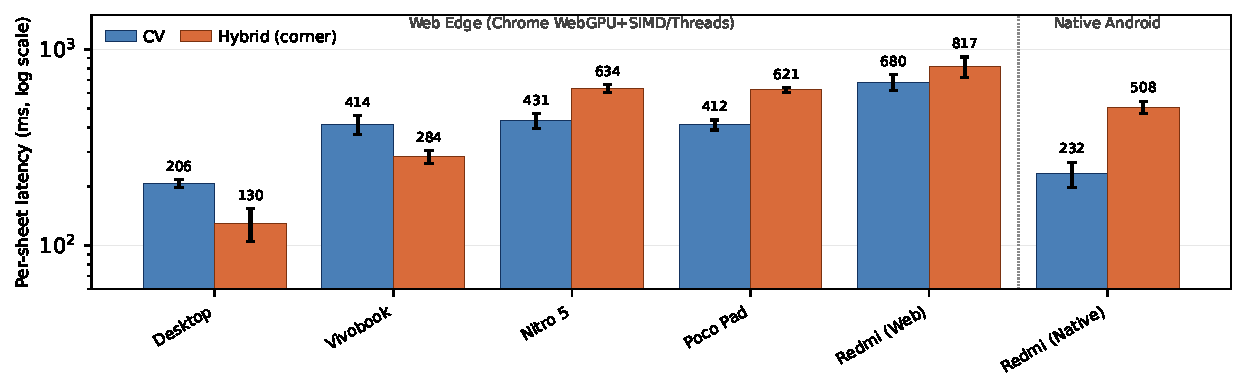
\includegraphics[width=\columnwidth]{figures/fig1_latency.pdf}
  \caption{Độ trễ mỗi phiếu theo nền tảng và cấu hình ($N{=}179$, thang
  log). Cột Web là \texttt{cpp\_ms}; cột Native là \texttt{e2e\_ms} dựa
  trên tệp.}
  \label{fig:latency}
\end{figure}

Toàn bộ ngân sách thời gian của Native củng cố sự quy gán này
(Bảng~\ref{tab:stage-mini}). Pipeline CV Native hoàn tất trong $108$\,ms
thời gian đầu-cuối dựa trên tệp, trong đó $77$\,ms là lõi C\texttt{++}
(\texttt{cpp}) còn phần còn lại là giải mã JPEG và một lần ghi gỡ lỗi,
trong khi pipeline YOLO Native hoàn tất trong $252$\,ms với NNAPI,
$360$\,ms trên bốn luồng CPU, và $470$\,ms trên một luồng. Số hạng chủ đạo
của nó là giai đoạn chuẩn hóa C\texttt{++} chứ không phải suy luận ONNX,
vốn có chi phí đo được là $150$\,ms dưới NNAPI. Native Android do đó vẫn
là phương án triển khai có độ trễ thấp hơn, nhưng không kèm độ chính xác
đã kiểm chứng theo chân trị, vì pipeline nhận dạng của nó chưa được căn
khớp với các nhãn đã rà soát và ở đây chỉ dùng làm mốc tham chiếu độ trễ
và tài nguyên. SIMD và đa luồng thu hẹp khoảng cách \wasm{} mà không xóa
bỏ nó: ngay cả khi bật cả hai, lõi CV Web vẫn chậm hơn vài lần so với đối
ứng bản địa, điều này một lần nữa xác định runtime \wasm{}, chứ không phải
bộ phát hiện, là yếu tố chi phối tính cạnh tranh của Web Edge.

Bên trong trình duyệt, hệ lai theo điểm-góc tái định hình cơ cấu chi phí
chứ không chỉ cộng thêm vào. Bảng~\ref{tab:hybrid} đối chiếu pipeline
chỉ-CV và pipeline theo điểm-góc trên bốn thiết bị tiêu biểu, mỗi cái báo
cáo dưới dạng trung vị năm lần chạy, và ba hiệu ứng lặp lại. Thứ nhất, hệ
lai nâng độ chính xác lên 99,43--99,44\% trên mọi thiết bị trong khi CV
giữ ở 99,00\%. Thứ hai, vì YOLO chạy trên GPU, hệ lai giảm gần một nửa mức
chiếm dụng CPU của tiến trình render, chẳng hạn từ $195\%$ xuống $91\%$
trên Vivobook và từ $158\%$ xuống $45\%$ trên Nitro~5. Thứ ba, thời gian
worker đầu-cuối tăng thêm một lượng gần như không đổi $\approx 300$\,ms,
là chi phí của suy luận WebGPU, nhưng bản thân \texttt{cpp\_ms} của
C\texttt{++} lại giảm trên các thiết bị yếu hơn vì đường theo góc bỏ qua
cả bước dò blob lẫn bước dò lại mốc lần hai, ví dụ từ $466$ xuống
$401$\,ms trên Redmi và từ $392$ xuống $234$\,ms trên Nitro~5. Như vậy hệ
lai đánh đổi một độ trễ cao hơn nhưng bị giới hạn bởi GPU lấy độ chính xác
cao hơn và áp lực CPU thấp hơn rõ rệt.

\begin{table}[t]
\caption{Chỉ-CV so với hệ lai theo điểm-góc trên bốn thiết bị ($N{=}179$,
trung vị năm lần chạy; threads + WebGPU).}
\label{tab:hybrid}
\centering
\scriptsize
\setlength{\tabcolsep}{3pt}
\resizebox{\columnwidth}{!}{%
\begin{tabular}{llccccc}
\toprule
\textbf{Thiết bị} & \textbf{Pipeline} & \textbf{ĐCX câu}
& \textbf{cpp} & \textbf{YOLO} & \textbf{worker} & \textbf{CPU/RAM đỉnh} \\
\midrule
Vivobook & CV     & 99,00\% & 308 & --  & 344 & 384\%/1889 \\
(laptop) & Lai    & \textbf{99,43\%} & 457 & 188 & 647 & 274\%/2523 \\
Nitro~5  & CV     & 99,00\% & 392 & --  & 451 & 217\%/1645 \\
(laptop) & Lai    & \textbf{99,43\%} & 234 & 482 & 718 & 247\%/1293 \\
Redmi    & CV     & 99,00\% & 466 & --  & 634 & 287\%/230 \\
(đt)     & Lai    & \textbf{99,43\%} & 401 & 541 & 944 & 174\%/253 \\
Poco Pad & CV     & 99,00\% & 332 & --  & 389 & 203\%/212 \\
(tablet) & Lai    & \textbf{99,44\%} & 250 & 444 & 695 & 119\%/240 \\
\bottomrule
\end{tabular}}
\vspace{2pt}
\parbox{\columnwidth}{\footnotesize
Thời gian tính bằng ms. Đơn vị CPU/RAM-đỉnh khác nhau theo công cụ (laptop
Windows: CPU\% tiến trình render và RSS-MB của \texttt{psutil}; Android:
bộ lấy mẫu trong ứng dụng, CPU\% trên thang $800$ và PSS-MB), nên CPU/RAM
chỉ nên so sánh trong cùng một thiết bị. ``Lai'' là bộ phát hiện YOLO theo
điểm-góc chạy trong trình duyệt trên WebGPU đưa vào một homography trực
tiếp.}
\end{table}

\begin{table}[t]
\caption{Độ trễ Native Redmi theo cấu hình ($N{=}179$, trung vị ms). Kiểm
chứng ngày 2026-06-19; nhận dạng chưa căn khớp chân trị (chỉ là mốc độ trễ).}
\label{tab:stage-mini}
\centering
\setlength{\tabcolsep}{4pt}
\resizebox{0.82\columnwidth}{!}{%
\begin{tabular}{lccc}
\toprule
\textbf{Cấu hình} & \textbf{Suy luận ORT} & \textbf{cpp} & \textbf{e2e} \\
\midrule
CV          & --  & 77  & 108 \\
YOLO NNAPI  & 150 & 224 & 252 \\
YOLO CPU-4T & 208 & 320 & 360 \\
YOLO CPU-1T & 321 & 433 & 470 \\
\bottomrule
\end{tabular}}
\vspace{2pt}
\parbox{\columnwidth}{\footnotesize
\texttt{cpp} là lõi OMR C\texttt{++}; \texttt{e2e} cộng thêm giải mã JPEG
và một lần ghi gỡ lỗi. ORT là thời gian suy luận ONNX Runtime đo được; các
giai đoạn chồng lấn với khâu chuẩn bị ảnh, nên các cột không cộng dồn một
cách chặt chẽ.}
\end{table}

\begin{table}[t]
\caption{Độ trễ Web (\texttt{cpp\_ms}) vòng đo trước cho các nền tảng chưa
đo lại theo giao thức điểm-góc. Bốn thiết bị có so sánh CV-vs-lai đã kiểm
chứng nằm ở Bảng~\ref{tab:hybrid} và Native Redmi ở
Bảng~\ref{tab:stage-mini}.}
\label{tab:latency}
\centering
\resizebox{0.92\columnwidth}{!}{%
\begin{tabular}{llcc}
\toprule
\textbf{Nền tảng} & \textbf{Ngăn xếp} & \textbf{CV (ms)} & \textbf{YOLO (ms)} \\
\midrule
Desktop tham chiếu & Win/Blink & $248\pm15$ & $246\pm18$ \\
Mac (M1)          & macOS/Blink & $240\pm16$ & $240\pm22$ \\
iPhone~16         & iOS/WebKit/chỉ SIMD & $\mathbf{160\pm14}$ & $\mathbf{165\pm18}$ \\
\bottomrule
\end{tabular}}
\vspace{2pt}
\parbox{\columnwidth}{\footnotesize
Ba nền tảng này được báo cáo từ vòng đo trước (CV và YOLO theo hộp bao) và
đang chờ đo lại theo giao thức điểm-góc. Cột YOLO ở đây là đường hộp bao,
không phải hệ lai theo điểm-góc của Bảng~\ref{tab:hybrid}. Thời gian thực
của trình duyệt Web không được các log batch xuất ra.}
\end{table}

\FloatBarrier

\subsection{Sử dụng tài nguyên hệ thống}
\label{sec:resources}

Mức tiêu thụ tài nguyên vẫn bị chặn trong suốt lượt chạy liên tục
(Bảng~\ref{tab:resources}, Hình~\ref{fig:cross_platform}), dù các con số
CPU phải đọc thận trọng vì đơn vị phụ thuộc công cụ: các hàng Windows báo
cáo CPU\% của tiến trình render, các hàng Mac, iOS và Android Web báo cáo
proxy vòng-lặp-sự-kiện trong trang, còn các hàng Native báo cáo một bộ lấy
mẫu Android theo thang $800\%$ trên SoC tám nhân. Đỉnh bộ nhớ Web lớn nhất
quan sát được là khoảng $1,3$\,GB, trên các máy desktop tham chiếu và lớp
Vivobook chạy Windows Chrome, trong khi bản dựng Native đạt đỉnh $514$\,MB
cho CV và $622$\,MB cho YOLO. Tuy các giá trị này chứng tỏ pipeline khả
thi trên phần cứng tầm trung, chúng cố ý không được trình bày như các tỉ
số hiệu suất CPU trực tiếp, vì không một công cụ đơn lẻ nào trải khắp mọi
nền tảng.

\begin{table}[!t]
\caption{Tóm tắt tài nguyên qua lượt chạy liên tục $N{=}179$. Ô CPU là
trung bình/đỉnh theo đơn vị gốc của công cụ; ô RAM là đỉnh CV/YOLO theo
MB.}
\label{tab:resources}
\centering
\scriptsize
\setlength{\tabcolsep}{2.5pt}
\resizebox{\columnwidth}{!}{%
\begin{tabular}{lcccl}
\toprule
\textbf{Máy} & \textbf{CPU CV} & \textbf{CPU YOLO}
& \textbf{RAM} & \textbf{Công cụ} \\
\midrule
Desktop & $60.5/168.7\%$ & $55.7/76.5\%$ & $1{,}310/984$ & psutil \\
Vivobook & $96.8/225.2\%$ & $85.3/156.9\%$ & $1{,}137/1{,}001$ & psutil \\
Nitro~5 & $74.7/204.6\%$ & $74.1/98.4\%$ & $1{,}145/1{,}071$ & psutil \\
M1 Mac & $0.59/0.89$ & $0.67/0.85$ & $1{,}073/248$ & proxy \\
iPhone~16 & $0.04/0.84$ & $0.21/0.83$ & $147/147$ & proxy \\
Poco Pad M1 & $169/203\%$ & $83/119\%$ & $212/240$ & sampler \\
Redmi Web & $202/287\%$ & $121/174\%$ & $230/253$ & sampler \\
Native & $341/431\%$ & $98/393\%$ & $514/622$ & sampler \\
\bottomrule
\end{tabular}}
\vspace{1pt}
\parbox{\columnwidth}{\footnotesize
Các máy Windows dùng CPU\% tiến trình render và RSS-MB của \texttt{psutil};
Mac/iPhone dùng proxy vòng-lặp-sự-kiện trong trang (Safari giấu telemetry
heap đầy đủ nên bộ nhớ là cận dưới); Android Web và Native dùng bộ lấy mẫu
adb/trong-ứng-dụng báo cáo CPU\% trên thang $800$ và PSS-MB. Cột CV/YOLO
của Android-Web là chỉ-CV so với hệ lai theo điểm-góc; YOLO Native là
provider NNAPI. Đơn vị không thể so sánh chéo giữa các công cụ.}
\end{table}

\begin{figure}[t]
  \centering
  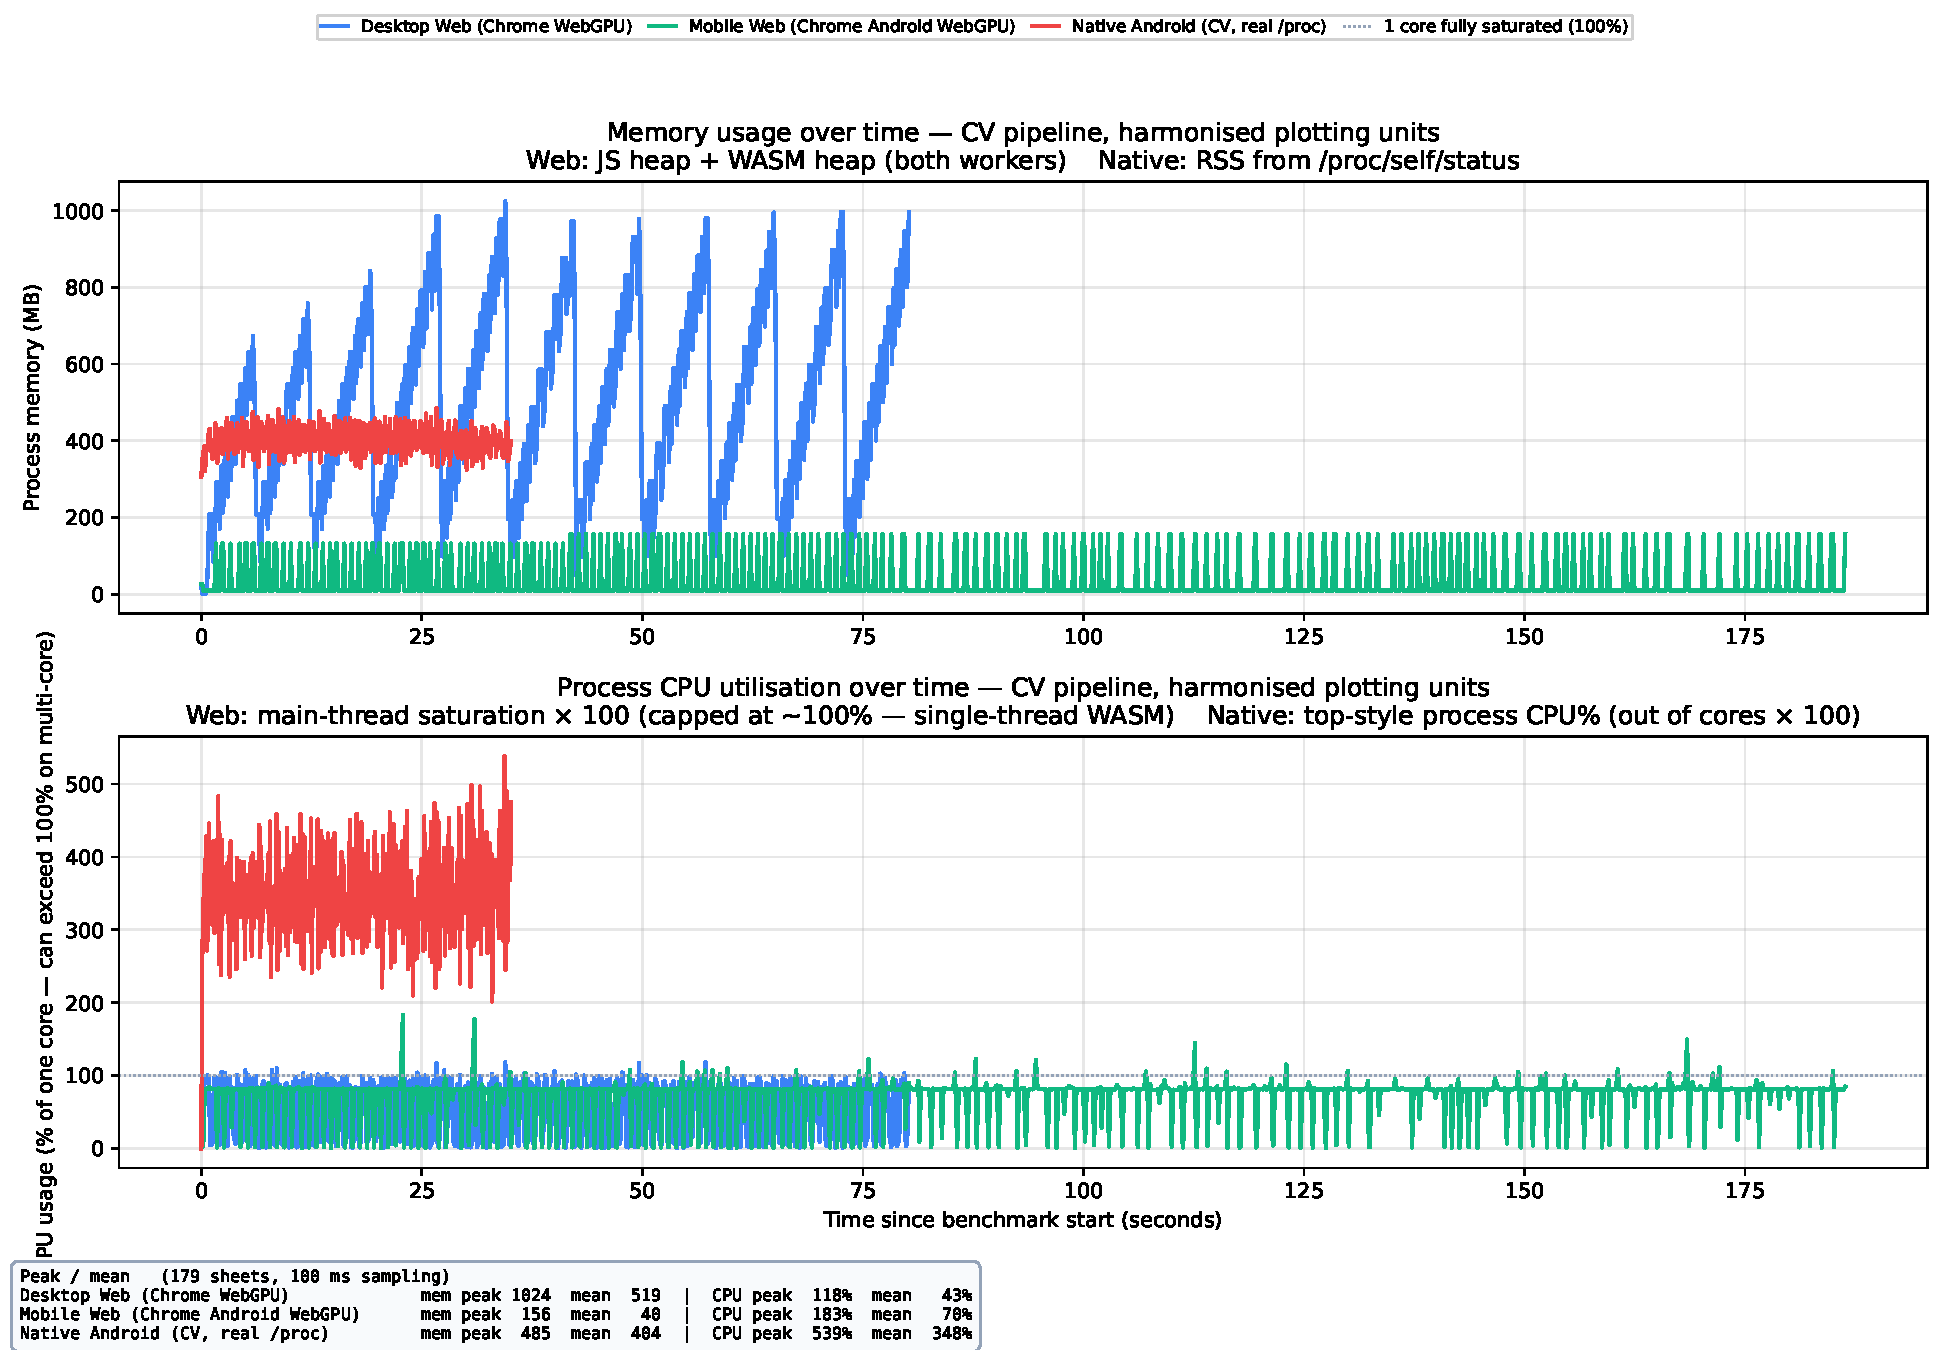
\includegraphics[width=\columnwidth]{figures/chart_cross_platform.pdf}
  \caption{Vết bộ nhớ và CPU kết hợp cho pipeline CV truyền thống. Bộ nhớ
  Web ổn định sớm, trong khi CPU Native dùng nhiều nhân theo từng đợt.}
  \label{fig:cross_platform}
\end{figure}

Các vết này cũng làm rõ vì sao một chỉ số CPU trình duyệt thấp hơn không
nên bị nhầm là thông lượng cao hơn. Worker Web có xu hướng nằm trong một
phong bì thực thi hẹp, gần như đơn nhân, chính vì lõi CV tất định được
biên dịch vào \wasm{} và tuần tự hóa qua mô hình bộ nhớ của nó, trong khi
OpenCV bản địa rút nhiều CPU lấy mẫu hơn nhưng biến những đợt bùng đó
thành độ trễ thấp hơn nhờ đa luồng bản địa và truy cập bộ nhớ trực tiếp.
Hàm ý nhất quán với phân tích độ trễ: mức tài nguyên bị chặn khẳng định
khả năng triển khai, nhưng tính cạnh tranh về độ trễ vẫn phụ thuộc vào
việc giảm chính chi phí CV trên \wasm{}.

\subsection{Các mối đe dọa đến tính hợp lệ}
\label{sec:threats}
\begin{enumerate}[label=(\roman*), leftmargin=*, itemsep=1pt, topsep=2pt]
  \item Các công cụ đo CPU/RAM khác nhau giữa các nền tảng, nên các giá
  trị tài nguyên được báo cáo theo đơn vị gốc của chúng và dùng để diễn
  giải xu hướng chứ không phải các tỉ số trực tiếp giữa các công cụ.
  \item Sản phẩm độ chính xác có giám sát phủ một bộ sưu tập 179 phiếu
  khuôn mẫu cố định. Đây là phạm vi khối lượng công việc dự kiến chứ không
  phải một tuyên bố về OMR bố cục tùy ý; dữ liệu tách biệt theo người viết
  và điều kiện chụp rộng hơn là phần kiểm định trong tương lai.
  \item Native Android chỉ là mốc độ trễ/tài nguyên. Web và Native dùng
  các giai đoạn thuật toán khớp ở mức mã nguồn, nhưng khác biệt về bản dựng
  OpenCV, thứ tự dấu phẩy động, bố cục bộ nhớ và pipeline cắt có thể làm
  thay đổi đầu ra nhận dạng; các nhãn YOLO theo từng câu của Native không
  được xuất ra trong benchmark hiện tại.
  \item Bộ phát hiện theo điểm-góc được huấn luyện trên 186 phiếu
  (mAP$@0.5\approx 0.99$ trên tập tách) rút từ một bộ sưu tập khuôn mẫu cố
  định, nên kết quả 99,43\% của nó được thiết lập cho bố cục này chứ không
  phải cho các mẫu tùy ý. Phép cắt-mask theo hộp bao vẫn là một lời cảnh
  báo rằng cùng bộ phát hiện vẫn có thể làm giảm chất lượng nhận dạng khi
  đầu ra của nó được tiêu thụ dưới dạng cắt thay vì dưới dạng các điểm góc.
  \item Độ trễ Web trên các laptop bị giới hạn nhiệt nhạy cảm với chế độ
  nguồn và trạng thái nhiệt của máy. Trên Vivobook (i5-13500H) chúng tôi
  quan sát được độ phân tán \texttt{cpp\_ms} mỗi phiếu lên tới
  $\approx 2\times$ qua các lần chạy High-Performance lặp lại, do điều
  tiết xung nhịp CPU/GPU chứ không phải thay đổi thuật toán (đầu ra nhận
  dạng giống hệt từng bit qua các lần chạy). Do đó mọi thiết bị trong
  Bảng~\ref{tab:hybrid} được báo cáo dưới dạng trung vị năm lần chạy, và so
  sánh Web-vs-Native được thực hiện trên cùng thiết bị Redmi để tránh yếu
  tố gây nhiễu này.
\end{enumerate}

\section{Kết luận}

OMR Web Edge cho thấy vừa chính xác vừa khả triển khai, song độ trễ của nó
được quyết định bởi cách các giai đoạn cân bằng chứ không phải bởi riêng
suy luận. Đường CV Web đã rà soát đạt độ chính xác câu hỏi 99,00\%, và một
bộ phát hiện YOLO theo điểm-góc đưa thẳng bốn điểm mốc dự đoán vào
homography nâng con số này lên 99,43\% trên bốn thiết bị, biến YOLO thành
một bộ định vị chính đã kiểm chứng; còn tiêu thụ cùng bộ phát hiện đó dưới
dạng cắt cứng lại khiến độ chính xác sụp còn 63,70--74,40\%, cho thấy chính
công thức, chứ không phải bộ phát hiện, mới là điều quan trọng. Về độ trễ,
một khi WebGPU đã hạ suy luận xuống chi phí thứ yếu, số hạng chủ đạo là
giai đoạn CV trên \wasm{}: trên cùng thiết bị Redmi, $466$\,ms của nó gấp
$6,1\times$ lõi bản địa $77$\,ms, một khoảng cách lớn hơn nhiều so với
$3,6\times$ giữa suy luận WebGPU và NNAPI. Native Android do đó vẫn là
phương án nhanh hơn, trong khi Web Edge đánh đổi độ trễ ấy lấy độ chính
xác đã kiểm chứng, quyền riêng tư và khả năng tiếp cận không cần cài đặt.
Thu hẹp khoảng cách còn lại rốt cuộc là vấn đề của việc tăng tốc CV qua
trình duyệt và một runtime \wasm{} tinh gọn hơn, chứ không phải một bộ
phát hiện nhanh hơn.

\begin{thebibliography}{11}

\bibitem{patel2015}
R.~Patel, S.~Sanghavi, D.~Gupta, and M.~S.~Raval,
``CheckIt: A low cost mobile OMR system,''
in \textit{Proc. IEEE TENCON}, 2015, pp.~1--6.

\bibitem{okorie2022}
U.~K.~Okorie, O.~Ezenwoye, and T.~H.~Kim,
``Robust image processing based real-time OMR system,''
in \textit{Proc. IEEE CSNT}, 2022, pp.~1--6.

\bibitem{afifi2019}
M.~Afifi and K.~F.~Hussain,
``The achievement of higher flexibility in multiple-choice-based tests
using image classification,''
\textit{IJDAR}, vol.~22, no.~2, pp.~91--126, 2019.

\bibitem{redmon2016}
J.~Redmon, S.~Divvala, R.~Girshick, and A.~Farhadi,
``You Only Look Once: Unified, real-time object detection,''
in \textit{Proc. IEEE CVPR}, 2016, pp.~779--788.

\bibitem{jocher2023}
G.~Jocher, A.~Chaurasia, and J.~Qiu,
``Ultralytics YOLOv8,'' 2023.
[Online]. Available: \url{https://github.com/ultralytics/ultralytics}

\bibitem{tabassum2024}
N.~Tabassum and M.~M.~Rahman,
``An efficient YOLOv8-based OMR system for automated answer sheet
grading,'' in \textit{Proc. ICCCI}, 2024, pp.~1--6.

\bibitem{ali2025}
M.~Ali, S.~Hammoud, and A.~Esper,
``Optical mark recognition techniques for multiple-choice tests:
A comprehensive review,''
\textit{IEEE Access}, vol.~13, pp.~156407--156423, 2025,
doi: 10.1109/ACCESS.2025.3600106.

\bibitem{microsoft2021}
Microsoft,
``ONNX Runtime Web,'' Sep.~2021.
[Online]. Available:
\url{https://opensource.microsoft.com/blog/2021/09/02/onnx-runtime-web-running-your-machine-learning-model-in-browser/}

\bibitem{jangda2019}
A.~Jangda, B.~Powers, E.~Berger, and A.~Guha,
``Not so fast: Analyzing the performance of WebAssembly vs.\ native
code,'' in \textit{Proc. USENIX ATC}, 2019, pp.~107--120.

\bibitem{wang2024}
Q.~Wang \textit{et al.},
``Anatomizing deep learning inference in web browsers,''
\textit{ACM Trans. Softw. Eng. Methodol.}, vol.~34, no.~2, Aug.~2024.

\bibitem{webnn2024}
W3C Machine Learning Working Group,
``Web Neural Network API,'' W3C Candidate Recommendation Draft,
21~May~2026.
[Online]. Available: \url{https://www.w3.org/TR/webnn/}

\end{thebibliography}

\end{document}
